%% LyX 2.3.3 created this file.  For more info, see http://www.lyx.org/.
%% Do not edit unless you really know what you are doing.
\documentclass[english]{article}
\usepackage[T1]{fontenc}
\usepackage[latin9]{inputenc}
\usepackage{float}
\usepackage{graphicx}

\makeatletter

%%%%%%%%%%%%%%%%%%%%%%%%%%%%%% LyX specific LaTeX commands.
%% Because html converters don't know tabularnewline
\providecommand{\tabularnewline}{\\}

%%%%%%%%%%%%%%%%%%%%%%%%%%%%%% User specified LaTeX commands.
\date{}

\@ifundefined{showcaptionsetup}{}{%
 \PassOptionsToPackage{caption=false}{subfig}}
\usepackage{subfig}
\makeatother

\usepackage{babel}
\begin{document}
\title{CSE 601 - Project 2 - Clustering Algorithms}
\author{Dipack P Panjabi (50291077), Krithika Srinivasan (-)}
\maketitle

\section{Overview}

This project focuses on implement 5 different clustering algorithms
- KMeans, Hierarchical Agglomerative clustering with Min approach,
density-based clustering, Gaussian mixture model clustering, and Spectral
clustering. These 5 clustering methods are tested on two provided
datasets, and their results are compared.

We use two external indexes to compare the clustering performance
of these algorithms, with the ground truth clusters - Rand Index,
and Jaccard Coefficient. We also visualise the resultant clusters,
by reducing their dimensions down to 2, using Principal Component
Analysis (PCA).

\section{Implementation}

\subsection{KMeans}

The KMeans algorithm is relatively simple to implement. The algorithm
is as follows:
\begin{enumerate}
\item From the given data, we select $n$ centroids, by selecting the first
$n$ data points, thereby giving us $n$ clusters.
\item We then assign each of the points in the data set to the cluster closest
to it, measured using Euclidean distance.
\item Once we have assigned all the points, we recompute the centroids of
each of the clusters, by averaging the coordinates of all the points
in the cluster.
\item Using the newly computed centroids, we repeat steps 2, and 3, until
we reach a point where the Euclidean distance between the old and
new cluster centroids is below a threshold, or, we have iterated a
enough times over the data set.
\end{enumerate}
\begin{figure}[H]
\subfloat[cho.txt]{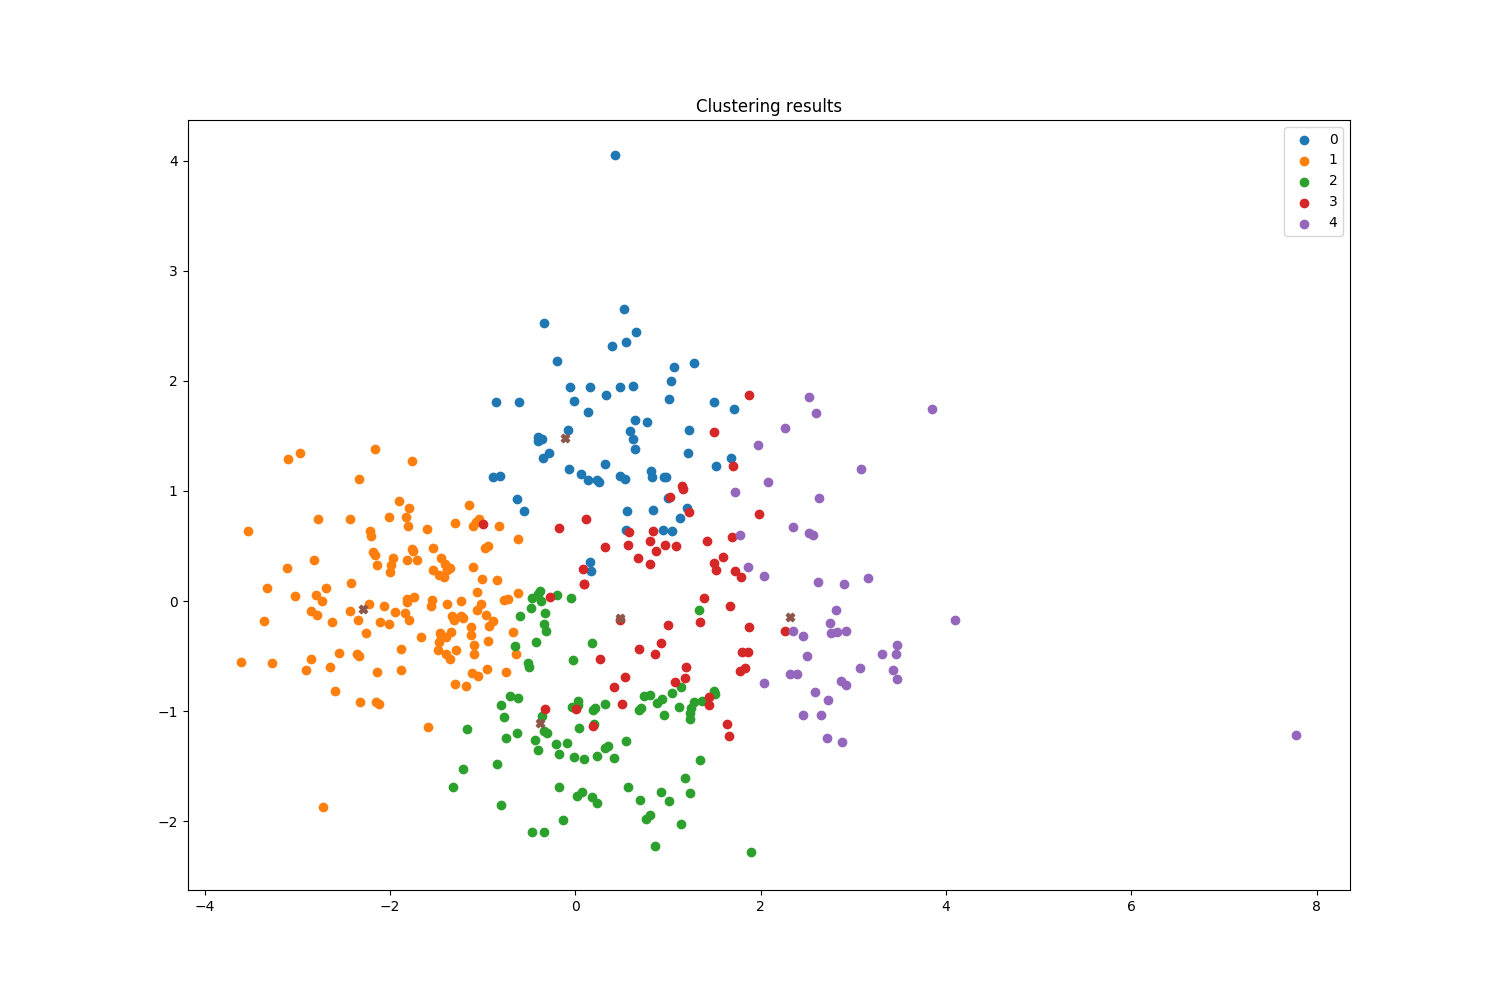
\includegraphics[scale=0.3]{images/cluster_kmeans_cho}

}\hfill{}\subfloat[iyer.txt]{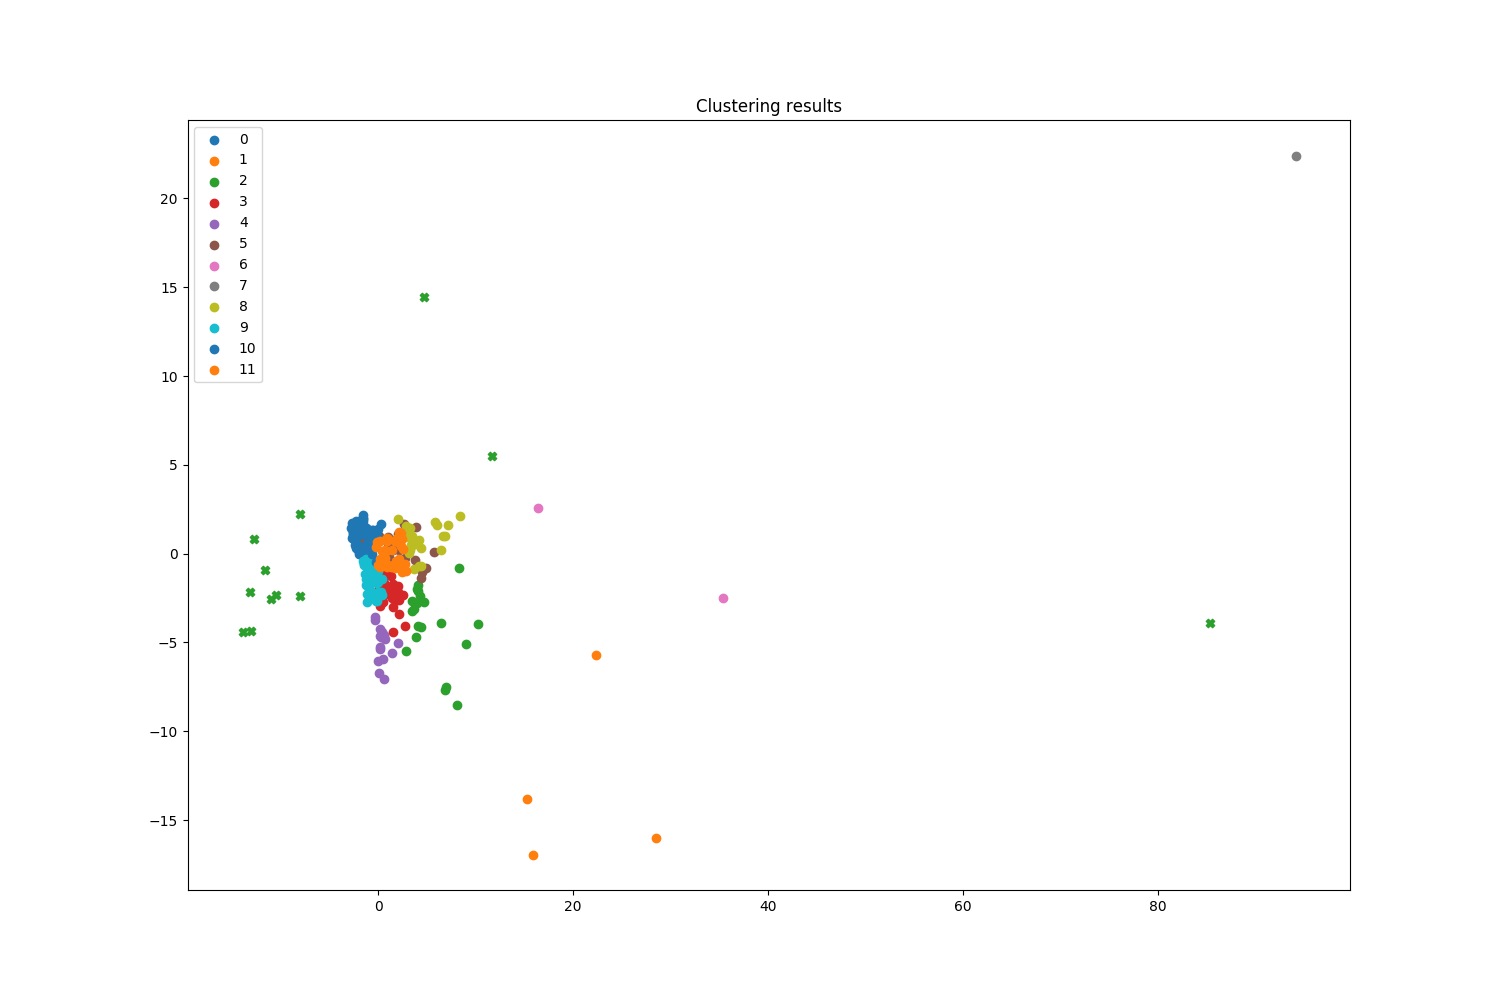
\includegraphics[scale=0.3]{images/cluster_kmeans_iyer}

}

\caption{KMeans clustering results}

\end{figure}

Figure 1 shows us the clusters computed by KMeans for each of the
two data sets. The cluster centroids are denoted as crosses - `x'.

\begin{table}[H]
\begin{tabular}{|c|c|c|}
\hline 
Dataset & Rand Index & Jaccard Coefficient\tabularnewline
\hline 
\hline 
cho.txt & 0.791 & 0.480\tabularnewline
\hline 
iyer.txt & 0.786 & 0.0174\tabularnewline
\hline 
\end{tabular}

\caption{KMeans clustering external index values}

\end{table}

Table 1 shows us the Rand Index, and Jaccard coefficient values for
the KMeans clusters generated for the two data sets.

From the table, we can see that both the Rand index, and Jaccard coefficient
are higher for the `cho.txt' data set, indicating that that particular
data set is better classified by KMeans. This is also corroborated
by the the data set visualizations in Figure 1, where the clusters
for `iyer.txt' are mostly clumped together, away from the actual data
points. A reason for this poor performance could be the fact that
KMeans has a tough time dealing with non-globular clustered data,
or data that has varying cluster densities. 

The advantages of KMeans, on the other hand, are exhibited quite nicely
by its performance on `cho.txt', which seems to be clustered quite
well, owing to the fact that most of the clusters have similar density,
and are spherically shaped in 2 dimensions.

\subsection{Hierarchical Agglomerative Clustering}

The hierarchical agglomerative clustering algorithm is as follows,
\begin{enumerate}
\item Each point in the given data is put into its own cluster, giving us
$n$ clusters for $n$ points.
\item We compute the inter-cluster distances, and use a Min Queue to store
them.
\begin{enumerate}
\item A Min Queue is a type of queue where the cluster pair with the shortest
distance is `popped'
\item The inter-cluster distance is computed by measuring the Euclidean
distance between between the two closest points between the two clusters.
\end{enumerate}
\item Once we have the two closest clusters in the current iteration, we
combine them to form a single cluster, replacing the two clusters,
and compute the inter-cluster distances again.
\item We repeat step 3, until we are left with the number of clusters we
want.
\end{enumerate}
\begin{figure}[H]
\subfloat[cho.txt]{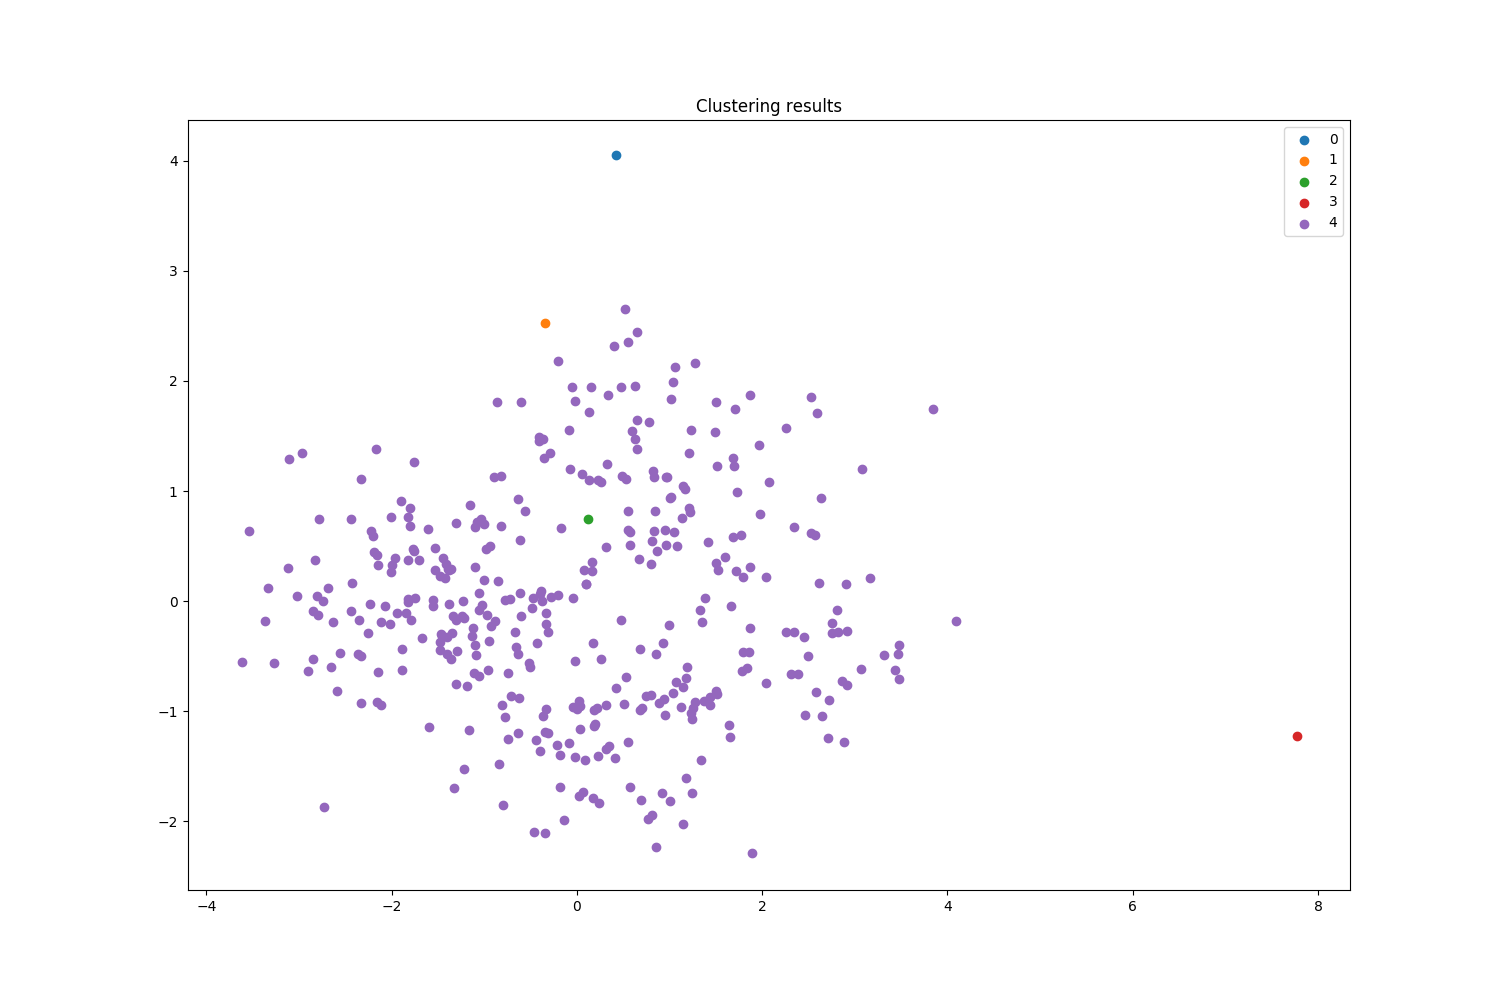
\includegraphics[scale=0.3]{images/cluster_hierarchical_cho}

}\hfill{}\subfloat[iyer.txt]{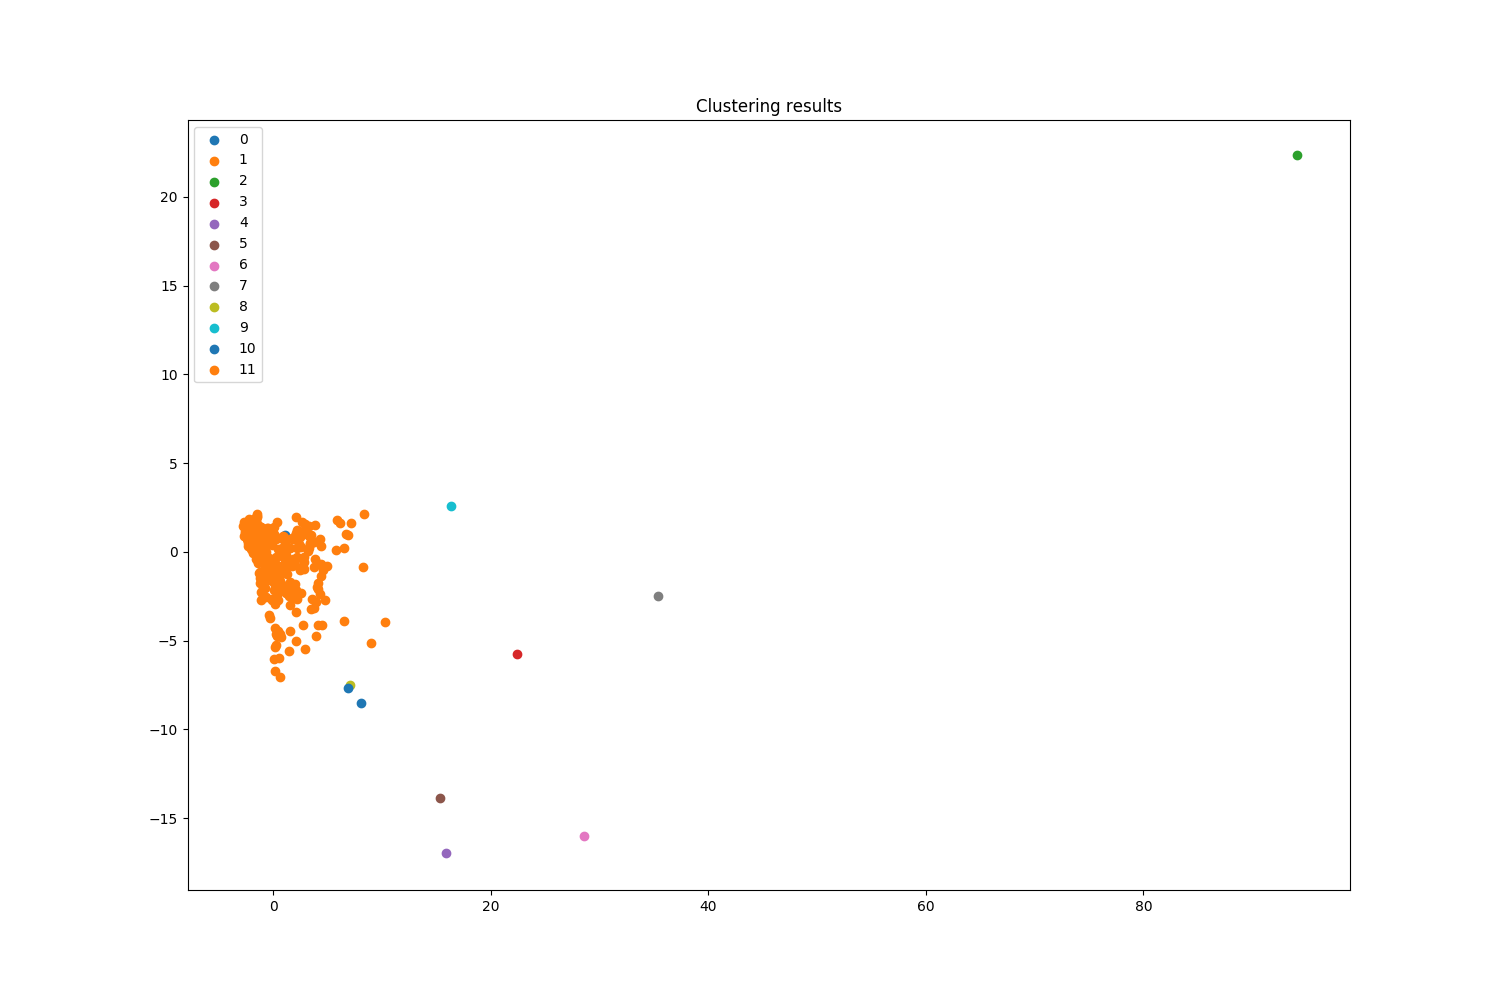
\includegraphics[scale=0.3]{images/cluster_hierarchical_iyer}

}

\caption{KMeans clustering results}
\end{figure}

Figure 2 shows us the hierarchical agglomerative clusters computed
for each of the two data sets.

\begin{table}[H]
\begin{tabular}{|c|c|c|}
\hline 
Dataset & Rand Index & Jaccard Coefficient\tabularnewline
\hline 
\hline 
cho.txt & 0.238 & 0.0252\tabularnewline
\hline 
iyer.txt & 0.192 & 0.00229\tabularnewline
\hline 
\end{tabular}

\caption{KMeans clustering external index values}
\end{table}

Table 2 shows us the Rand Index, and Jaccard coefficient values for
the hierarchical agglomerative clusters generated for the two data
sets.

As the results show us, we get a `mega' cluster for both data sets,
with all the remaining clusters consisting of just a single point
each. The external index results show us that while we do classify
certain points correctly, the overwhelming majority of points are
misclassified. We can conclude that this algorithm performs very poorly,
compared to KMeans, as it is quite sensitive to noise and outlying
points.

An advantage of this clustering technique is the fact that it can
identify and deal with non-elliptical cluster formations.
\end{document}
